%\section{Entwicklung eines konzeptuellen Rahmens}
\section{Vorgehensmodell für Cloud-Migrationen}
\label{cha:entwicklung_vorgehensmodell}
In diesem Kapitel wird ein dreistufiges Vorgehensmodell (vgl. 
Abbildung~\ref{fig:vorgehensmodell}) für Cloud-Migrationen entwickelt, das sich 
an ISV mit ihren Bedürfnissen und Anforderungen 
richtet.
%\documentclass[border=10pt]{standalone}

\usetikzlibrary{decorations.text}
\usetikzlibrary{calc}
\usetikzlibrary{fit}
\usetikzlibrary{shapes}
\usetikzlibrary{arrows,positioning} 
\pgfmathsetmacro{\cubex}{4}
\pgfmathsetmacro{\cubey}{2}

\definecolor{light-gray}{gray}{0.80}

\tikzset{
    %Define standard arrow tip
    >=stealth',
    %Define style for boxes
    punkt/.style={
           rectangle,
           rounded corners,
           draw=black, very thick,
           text width=7em,
           minimum height=2em,
           text centered},
    % Define arrow style
    pil/.style={
           ->,
           very thick,
           shorten <=5pt,
           shorten >=5pt,},
}




%\begin{document}
\begin{figure}[bh]
\begin{center}
\begin{tikzpicture}




% Punkte
\newcommand{\boxNO}{(0,0)}
\newcommand{\boxNW}{(-\cubex,0)}
\newcommand{\boxSO}{(0,-\cubey)}
\newcommand{\boxSW}{(-\cubex,-\cubey)}


% On-Premise-Produkt
\draw[black,fill=light-gray,very thick] \boxNW -- \boxNO -- \boxSO -- \boxSW -- 
cycle;
\draw (-0.5*\cubex,-0.5*\cubey) node {\textbf{On-Premise-Produkt}};

% Trichter
\newcommand{\trichterBreiteO}{1.5*\cubex}
\newcommand{\trichterBreiteM}{0.33*\cubex}
\newcommand{\trichterAbstand}{0.5*(\trichterBreite - \trichterBreiteM)}

\newcommand{\trX}{-1.25*\cubex}
\newcommand{\trY}{-1.25*\cubey}
\newcommand{\trichterNW}{ (\trX, \trY) }
\newcommand{\trichterNO}{ (\trX+\trichterBreiteO, \trY) }

\newcommand{\trichterMW}{ ( \trX + 0.33*\trichterBreiteO, \trY-0.75*\cubey ) }
\newcommand{\trichterMO}{ ( \trX + 0.66*\trichterBreiteO, \trY-0.75*\cubey ) }

\newcommand{\trichterSW}{ ( \trX + 0.33*\trichterBreiteO, \trY-1.75*\cubey) }
\newcommand{\trichterSO}{ ( \trX + 0.66*\trichterBreiteO, \trY-1.75*\cubey) }

\newcommand{\trichterC}{ ( \trX + 0.5*\trichterBreiteO, \trY-0.5*0.75*\cubey) }

\draw[black,thick] %,fill=SkyBlue 
	\trichterNW -- 
	\trichterNO -- 
	\trichterMO --
	\trichterSO --
	\trichterSW --
	\trichterMW --
	\trichterNW;
% Uncomment for text in Trichter
%\draw \trichterC node {};


% Diamond



\newcommand{\diamondX}{\trX + 0.5*\trichterBreiteO}
\newcommand{\diamondY}{\trY-2.3*\cubey}
%star point height=.9cm, minimum size=0.7*\cubey,draw,
\node [starburst, fill=Goldenrod,draw,starburst points=13] (VISION)
at (\diamondX,\diamondY) {Vision};
	
\newcommand{\boxREx}{\diamondX}
\newcommand{\boxREy}{\diamondY - 1.2*\cubey}
\newcommand{\boxRo}{1.8*\cubey}
\newcommand{\boxRm}{2*\cubey}
\newcommand{\boxRu}{1.2*\cubey}
\newcommand{\boxHEins}{.9*\cubey}
\newcommand{\boxHZwei}{2*\cubey}
\newcommand{\boxHDrei}{3*\cubey}


 \node[punkt] (RE) at (\boxREx,\boxREy) {Requirements Engineering} ;  
\node[punkt] (PL) at (\boxREx-\boxRo,\boxREy -\boxHEins)  {Planning}
 edge[pil] (RE.west) ;
 
 \node[punkt] (EVAL) at (\boxREx-\boxRm,\boxREy -\boxHZwei)  {Evaluation} 
edge[pil] (PL.south);
 
 
 \node[punkt] (T) at (\boxREx-\boxRu,\boxREy -\boxHDrei)  {Testing}
 edge[pil] (EVAL.south) ;
 
 
 \node[punkt] (DEPL) at (\boxREx+\boxRu,\boxREy -\boxHDrei)  {Deployment}
 edge[pil] (T.east);
 
 
 \node[punkt] (I) at (\boxREx+\boxRm,\boxREy -\boxHZwei)  {Implementation}
 edge[pil] (DEPL.north);
 
 \node[punkt] (AD) at (\boxREx+\boxRo,\boxREy -\boxHEins)  {Analysis \& Design}
edge[pil] (I.north);

\draw[pil]
  (RE.east) edge (AD.north);
  
\draw[pil] (VISION) edge (RE.north);

 
\node [cloud, draw,cloud puffs=10,cloud puff arc=120, aspect=2, inner 
ysep=3*\cubex,fill=Goldenrod] (CLOUD) at (\boxREx,\boxREy-0.8*\boxHZwei) 
{\textbf{Cloud L\"osung}};
 
 
 %\node[punkt, inner sep=5pt,below=0.5cm of RE]
 %(formidler) {Intermediaries (c)};
 % We make a dummy figure to make everything look nice.
 %\node[above=of RE] (dummy) {};
 %\node[right=of dummy] (t) {Ultimate borrower}
  %edge[pil,bend left=45] (RE.east) % edges are used to connect two nodes
  % edge[pil, bend left=45] (I.east); % .east since we want
                                             % consistent style
 %\node[left=of dummy] (g) {Ultimate lender}
   %edge[pil, bend right=45] (RE.west)
   %edge[pil,<->, bend left=45] node[auto] {Direct (a)} (t);
	
\end{tikzpicture}
\caption{Darstellung des Vorgehensmodells. Der iterative Software Engineering 
Kreislauf wurde \cite{changes_in_requirements_engineering} entnommen.}
\label{fig:vorgehensmodell}
\end{center}
\end{figure}

%\end{document}



Das Vorgehen in jeder Phase ist von dem grundlegenden Ziel geprägt, Chancen der 
Cloud zu realisieren und spezifische Risiken zu vermeiden. Deshalb werden 
zunächst Chancen und Risiken identifiziert und daraus resultierenden 
Fragen, Problemstellungen und Herausforderungen vorgestellt, deren 
Beantwortung den ISV beim Meistern der Migration unterstützen. Die 
Reihenfolge, in der Chancen und Risiken betrachtet werden, hat keine 
Bedeutung. 

Nicht alle Chancen und Risiken entstehen exklusiv und unbedingt 
bei der Cloud-Nutzung. Deshalb ist auch ein Vergleich mit der Situation in der 
bestehenden On-Premise Situation erforderlich. Um der Cloud mit ihren Chancen 
und Risiken bestmöglich zu begegnen sind auch weitreichende Änderungen am 
Unternehmen selbst zu berücksichtigen.

In Phase I wird anhand des bestehenden On-Premise-Produktes eine Vision 
geformt, die unter Umständen einen sehr viel kleineren Funktionsumfang als die 
On-Premise-Software aufweisen wird. Dabei werden aber Chancen und Risiken des 
Cloud-Marktes berücksichtigt und so Wettbewerbsfähigkeit und ein schneller 
Markteintritt ermöglicht. 

Anschließend wird in Phase II die Machbarkeit der Vision in technischer und 
wirtschaftlicher Hinsicht geprüft. Maßgeblich ist die Frage, ob innerhalb 
eines bestimmten Kostenrahmens auf gegebener
Plattform ein konkurrenzfähiges Produkt geschaffen werden kann.

Schließlich wird die Vision in Phase III in einem an die Cloud 
angepassten, agilen, iterativen Entwicklungsprozess realisiert. Es wird 
gezeigt, in welchen Aspekten bekannte agile Modelle angepasst werden müssen, um 
mit der besonders hohen Geschwindigkeit der Cloud Schritt halten zu können. 

Bevor sie im Detail vorgestellt wird, wird jede Phase zunächst begründet 
und zur Orientierung vom Fünf-Phasen-Modell abgegrenzt.
\begin{comment}
Das Fünf-Phasen-Modell beginnt mit einer technischen und 
wirtschaftlichen Machbarkeitsstudie. Die Migration einer On-Premise-Software in 
die Cloud bedeutet für das migrierende Unternehmen die Erschließung eines ganz 
neuen Marktes, der sich grundlegend vom bekannten Markt unterscheidet. Aus 
diesem Grund kann das Cloud-Produkt sich grundlegend vom bisherigen 
On-Premise-Produkt unterscheiden. Deshalb wird 
\citeflow{how_saas_changes_an_isvs_business} und 
\citeflow{towards_modelling_a_cloud_applications_life_cycle} eine zusätzliche 
Phase vorgeschlagen, in der eine Vision der künftigen Cloud-Lösung entworfen 
wird. Mit dieser Vision kann der Leistungsumfang abgeschätzt werden und auch, 
wie sich das Unternehmen verändern muss, um dieser Vision zu entsprechen. 
(Kapitel~\ref{cha:phaseI})\\
\end{comment}

\subsection{Chancen der Cloud}
Die folgenden Chancen der Cloud wurden bei der Literaturrecherche identifiziert:
\begin{table}[ht!]
\centering
\begin{longtable}{|p{0.15\textwidth}|p{0.38\textwidth}|p{0.38\textwidth}|}
\hline
\textbf{Bezeichnung} & \textbf{Beschreibung \& Quelle} & \textbf{Fragen \& 
Aufgaben für den ISV} \\
\hline %%%%%%%%%%%%%%%%%%%%%%%%%%%%%%%%%%%%%%%%%%%%%%%%%%%%%%%%%%%%%%%%%
Soziales Element & Das soziale Element entsteht durch neue Möglichkeiten 
des Austausches, die durch die Nutzung einer gemeinsamen Cloud-Plattform 
entstehen: zwischen Nutzern innerhalb eines Unternehmens, zwischen 
verschiedenen Unternehmen oder mit den Entwicklern. Die Weiterentwicklung wird 
dadurch inklusiver, Nutzer lassen sich einbeziehen. 
\pcite{}{}{cloud_based_next_generation_service_and_key_challenges, 
changes_in_requirements_engineering} &
Wie lässt sich der Kontakt zu und zwischen Kunden und ihren Fachabteilungen so 
direkt, einfach und produktiv wie möglich gestalten? Lassen sich Communities 
aufbauen? \\
\hline %%%%%%%%%%%%%%%%%%%%%%%%%%%%%%%%%%%%%%%%%%%%%%%%%%%%%%%%%%%%%%%%%
Analyse\-möglich\-keiten & Da sich alle Benutzer auf der Cloud 
bewegen, fallen viel mehr Informationen an, die analysiert werden können
\pcite{}{}{cloud_based_next_generation_service_and_key_challenges,
changes_in_requirements_engineering} & Wie lassen 
sich künftige Entscheidungen mit den gewonnenen Informationen fundierter 
treffen? \\
\hline %%%%%%%%%%%%%%%%%%%%%%%%%%%%%%%%%%%%%%%%%%%%%%%%%%%%%%%%%%%%%%%%%
Mobilität & Lösungen aus SaaS-Bereich sind häufig bereits im Standard auf 
mobile Bedienbarkeit 
ausgelegt. \pcite{}{}{cloud_based_next_generation_service_and_key_challenges} & 
Um bezüglich Mobilität nicht nur Erwartungen zu erfüllen, sondern 
Begeisterung zu wecken, sollte geprüft werden, wie die gewonnene Mobilität im 
konkreten Fall den Kundenwert steigern kann. \\
\hline %%%%%%%%%%%%%%%%%%%%%%%%%%%%%%%%%%%%%%%%%%%%%%%%%%%%%%%%%%%%%%%%%
Reduzierte Markteintrittskosten \& Skalierte Märkte & Durch pay-per-use-Modelle 
sind die Markteintrittskosten drastisch reduziert.
\pcite{}{}{cloud-computing_the_business_perspective} & Mit welchen Produkten 
lassen sich neue Märkte erschließen? Welche unerschlossenen Märkte gibt es? Wie 
lassen sich geographisch weit entfernte Märkte erschließen? \\
\hline %%%%%%%%%%%%%%%%%%%%%%%%%%%%%%%%%%%%%%%%%%%%%%%%%%%%%%%%%%%%%%%%%
Skalierung der Leistung & In der Cloud stehen -- dynamisch an den aktuellen 
Bedarf angepasst -- unbegrenzte Ressourcen bereit.
\pcite{}{}{cloud-computing_the_business_perspective} & Wie lassen sich die 
Ressourcen nutzen, um gegenüber On-Premise-Anwendungen im Vorteil zu sein? \\
\hline %%%%%%%%%%%%%%%%%%%%%%%%%%%%%%%%%%%%%%%%%%%%%%%%%%%%%%%%%%%%%%%%%

Time to market \& kürzere Releasezyklen & 
Die Software und auch Updates lassen sich schneller auf den Markt bringen. 
\pcite{}{}{changes_in_requirements_engineering} &
\\
\hline

Alternativen testen & 
In der Cloud lassen sich alternative Implementierungen 
testen und direkt auswerten. \pcite{}{}{changes_in_requirements_engineering} &
\\ \hline

Sparen der Wartung älterer Versionen & 
Kapazitäten werden frei, da es in der Cloud nur eine aktuelle Version gibt, in 
die alle Entwicklungsarbeit fließen kann und keine Altversionen gewartet und 
berücksichtigt werden müssen. \pcite{}{}{changes_in_requirements_engineering, 
transitioning_to_saas} &
\\ \hline
\end{longtable}
\caption{Chancen durch die Migration in die Cloud}
\label{tab:chancen_der_cloud}
\end{table}
\addtocounter{table}{-1}


\subsection{Risiken der Cloud}
Die folgenden Risiken der Cloud wurden bei der Literaturrecherche identifiziert:
\begin{table}[ht!]
\centering
\begin{longtable}{|p{0.11\textwidth}|p{0.4\textwidth}|p{0.4\textwidth}|}
\hline
\textbf{Stichwort} & \textbf{Beschreibung \& Quelle} & \textbf{Fragen \& 
Aufgaben für den ISV} \\
\hline %%%%%%%%%%%%%%%%%%%%%%%%%%%%%%%%%%%%%%%%%%%%%%%%%%%%%%%%%%%%%%%%%

\hline %%%%%%%%%%%%%%%%%%%%%%%%%%%%%%%%%%%%%%%%%%%%%%%%%%%%%%%%%%%%%%%%%
\end{longtable}
\caption{Mögliche Risiken durch die Migration in die Cloud}
\label{tab:risiken_der_cloud}
\end{table}



\subsection{Phase I: Entwicklung einer Vision}
\label{cha:phaseI}

Als "`disruptive innovation"' ist die Cloud auch ein neuer Markt, auf dem 
qualitativ hochwertige, teilweise hoch spezialisierte IT-Dienstleistungen 
gehandelt werden \pcite{}{}{towards_modelling_a_cloud_applications_life_cycle}. \\
Durch das pay-per-use-Preismodell sind auch kleine Unternehmen in der Lage, 
diese Technologien und Dienstleistungen zu nutzen 
\pcite{}{156}{cloud_migration}. Dementsprechend ist die Nutzung der Cloud im Vergleich zum Wettbewerb per se 
weder  innovativ -- da jeder die Technologie nutzen kann -- noch 
automatisch ein Wettbewerbsvorteil: Sie ist ein wirtschaftliches Erfordernis, 
um den Wettbewerb nicht zu verlieren 
\pcite{}{}{challenges_of_cloud_computing_in_business}.

Um mit der Cloud-Migration nicht nur dieses wirtschaftliche Erfordernis zu bewältigen, sondern 
einen Wettbewerbsvorteil zu erringen, muss nach der Migration ein Wert für den 
Kunden geschaffen sein. Die Software muss unter aktuellen und möglichen 
zukünftigen Konkurrenten einzigartig oder wenigstens selten sein, annähernd 
unnachahmlich und schwer substituierbar sein 
\pcite{}{}{theoretical_perspectives_for_strategic_human_resource_management}.
Es bedarf der geschickten Integration standardisierter, in der Cloud 
verfügbarer Komponenten zu einer innovativen Gesamtlösung. 
%Gelingt dies nicht, ist eine Differenzierung von 
%konkurrierenden, sich gleichenden Produkten nur über einen niedrigeren Preis 
%möglich. \pcite{}{}{towards_modelling_a_cloud_applications_life_cycle} \\

\citeflow{fivephases} gehen in ihrem Fünf-Phasen-Modell von einer vollständigen 
Migration mit der Gesamtheit aller Funktionalität aus. Davon wird in dem hier 
vorgestellten Modell bewusst abgewichen. Bei einer vollständigen Migration 
dauert es, aufgrund der höheren Entwicklungsdauer, länger, bis Umsätze generiert 
werden. Benötigte Investitionen steigen immens und mit ihnen das Risiko. Des 
Weiteren wäre es mit einer 1:1-Migration weder möglich die Chancen der 
Cloud zu realisieren, noch die Risiken zu umschiffen. Dies betrifft das 
Produkt selbst -- so kann es beispielsweise versäumt werden, zu bedenken, wie 
mobile Nutzung einen besonderen Wert für den Kunden schaffen kann -- aber auch 
den Entwicklungsprozess. Möglichkeiten, wie die der schnellen, unkomplizierten 
Releases und der frühen Nutzerrückmeldung und die besondere Agilität die sich 
daraus gewinnen lässt, werden verschenkt.

Aus diesen Gründen wird eine sprintweise Migration und 
Weiterentwicklung vorgeschlagen, die mit der Vision eines Produktes beginnt. 
Das Verständnis des Begriffes "`Produktvision"' ist ein strategisches und wurde 
aus den Eigenschaften abgeleitet, die \citeflow{the_power_of_vision} 
Unternehmensvisionen zuschreiben.

Um ein wettbewerbsfähiges Produkt zu schaffen, sollte eine Produktvision die genannten Chancen und Risiken - angelehnt an die Methode der SWOT-Analyse %Seiten 501,6
\pcite{}{}{marketingmanagement,cloud-computing_the_business_perspective} - berücksichtigen. 
Sie sollte klar und deutlich sein, den Umfang des Produktes so klein wie möglich, doch so umfangreich wie nötig halten, 
um frühestmöglich ein auslieferbares, begeisterndes Produkt zu schaffen. Dennoch sollte die Vision dabei stabil, 
zukunftsorientiert und langfristig ausgelegt sein, sie sollte herausfordernd aber erreichbar sein. Formulierte Produkteigenschaften müssen abstrakt genug sein, um Freiheiten bei der Umsetzung zu lassen. 

Damit die Vision realisiert werden kann, müssen Prozesse und 
Unternehmensorganisation an ihr ausgerichtet werden. Sie muss kommuniziert und Mitarbeiter in die Lage versetzt werden, sie zu erreichen \pcite{}{}{the_power_of_vision}.

Die Vision muss auch Einfluss auf das Geschäftsmodell nehmen. Gerade beim 
Auftreten von "`disruptives innovations"' scheitern viele Unternehmen, 
weil sie nicht in der Lage oder willens sind, ihr Geschäftsmodell in 
ausreichendem Maße zu ändern 
\pcite{}{}{disruptive_technologies_a_business_model_perspective}. Um ein 
wirtschaftlich nachhaltiges, an die Realitäten des Marktes angepasstes, 
wettbewerbsfähiges Geschäftsmodell für den Cloud-Markt zu entwickeln, sollte 
der ISV unter Berücksichtigung der Chancen und Risiken die folgenden Fragen 
beantworten \pcite{}{}{disruptive_technologies_a_business_model_perspective}:
\begin{enumerate}
	\item Wie entsteht für den Kunden Wert in Form eines Produktes oder 
		einer Dienstleistung?
	\item In welcher Form und Höhe und mit welchem Preismodell wird Umsatz 
generiert? 
	\item Wie können bereits bestehende und kommende standardisierte 
Komponenten und Dienstleistungen in das Produkt integriert werden?
	\item Wie lassen sich bestehende oder zu erwerbende Ressourcen und 
Fähigkeiten (andersartig) nutzen, um neue Produkte oder Dienstleistungen zu 
erzeugen?
	\item Mit welchen strategischen Entscheidungen lassen sich 
Wettbewerbsvorteile (auch gegenüber On-Premise-Lösungen und 
zugehörigen Preismodellen) erlangen?
\end{enumerate}

\begin{comment}
Aus \citeflow{the_power_of_vision}:
\begin{itemize}
	\item Notwendigkeiten um Vision zu realisieren: \\
	\begin{itemize}
		\item communicating the vision
		\item aligning organizational processes and systems to suit the 
vision
		\item empowering others to act to achieve the vision
		\item motivating staff
	\end{itemize}
	\item Charakterisitika eng mit Unternehmenserfolg verbunden


\end{itemize}
\end{comment}
%\subsubsection{TODO: Preismodell}


%Aus einer technologischen Innovation wird für ein Unternehmen erst ein Wert, 
%wenn es mit einem erfolgreichen Geschäftsmodell vermarktet werden kann.



\begin{comment}
\subsubsection{Organisationsstruktur}
Da der Kunde des ISV keine Serverinfrastruktur betreiben muss, um die 
Cloud-Lösung zu nutzen und auch auf den Rechnern der Endbenutzer nichts 
installiert werden muss, entfallen im Idealfall Verhandlungen zwischen ISV und 
der IT-Abteilung des Kunden; Entscheidungen werden in kleineren Kreisen, direkt 
von Fachabteilungen getroffen. Für den ISV hat dies zur Folge, dass er mit 

Als Abstraktionsschicht ermöglicht es Cloud-Computing Unternehmen die 
Wertschöpfungskette zu verschlanken und sich auf ihr Kerngeschäft zu 
konzentrieren.

Cloud-Computing wird im Ideal als Abstraktionsschicht gesehen, die 
Komplexitäten 
vor Fachabteilungen und Führungskräften verbirgt und es ihnen ermöglicht ohne 
Entwickler. Wo in der Vergangenheit Empfehlungen, Design, Entwicklung, 
Deployment und Wartung in den Händen von IT-Abteilungen lagen, ist es im 
Cloud-Computing nötig, dass Führungskräfte

Auf dem Weg zum einzigartigen, innovativen und wettbewerbsfähigen Produkt, muss 
sich ein Unternehmen auf seine Kernkompetenzen konzentrieren und 
das Thema IT neu betrachten, um die Flexibilität und Agilität der Cloud nutzen 
zu können. Anstatt sich in der Hauptsache die bestehende 
IT-Infrastruktur zu unterhalten, werden IT-Abteilungen zu strategischen 
Partnern 
in der Weiterentwicklung der Produkte 
\pcite{}{}{how_saas_changes_an_isvs_business}: Mitarbeiter aus der IT müssen 
genutzt werden, um qualitativ hochwertige, nutzbare 
Trends bei Cloud-Dienstleistungen frühzeitig zu erkennen und kreativ in das 
Produkt einfließen zu lassen oder Business-Prozesse bestmöglich zu 
unterstützen.
\end{comment}


\begin{comment}

\subsection{Phase I: Business, Strategie und Struktur neu gestalten}

\subsubsection{IT-Strategie}
Unter einer IT-Strategie 
verstehen \citeflow{
towards_an_understanding_of_cloud_computings_impact_on_org_it_strategy} die 
organisationsweite Perspektive auf Investitionen in IT-Systeme sowie das 
Deployment, die Nutzung und das Management von IT-Systemen. Die IT-Strategie 
legt insbesondere fest
\begin{itemize}
	\item welchen Umfang die IT im Unternehmen hat
	\item welche IT-Fähigkeiten vorgehalten werden
	\item wie Steuerung und Controlling erfolgen
	\item wie das Anwendungsportfolio zusammengestellt ist
	\item wie Daten verarbeitet und gespeichert werden
	\item wie IT und Business aufeinander abgestimmt werden
\end{itemize}
\citeflow{
towards_an_understanding_of_cloud_computings_impact_on_org_it_strategy} 
identifizieren einige Auswirkungen einer Cloud-Migrationen auf die IT-Strategie 
für Unternehmen. Aus den allgemein gehaltenen Auswirkungen, werden Vorschläge 
abgeleitet, die sich an Independent Software Vendors richtet.
\begin{description}.
\end{description}

\begin{comment}
Hauptmotivation die Cloud zu Nutzen, sollte nicht die Reduktion von Kosten
sein, sondern strategische Vorteile, wie eine Konzentration auf das
Kerngeschäft, schnellere und effizientere Innovationsprozesse,
Produktivitätssteigerungen und eine IT, die das Business besser unterstützt,
womöglich sogar profitabel ist. \pcite{}{}{the_strategic_value_of_the_cloud}

Gerade weil die Migration in die Cloud große technische aber vor allem auch
geschäftliche Umwälzungen mit sich bringt, sollte die Migration wirtschaftlich
begründet werden, genauer gesagt:
strategisch. \pcite{}{}{challenges_and_assessment_in_migrating} Auch wenn die
Nutzung der Cloud Einsparungen ermöglicht, machen IT-Budgets in der Regel
nur einen geringen Prozentsatz des Umsatzes aus. Hauptmotivation für die
Migration in die Cloud sollten deshalb strategische Ziele sein, mit denen der
Umsatz ausgebaut oder zumindest behauptet wer
\end{comment}

\begin{comment}
\subsubsection{SWOT-Analyse}
Aus \pcite{}{}{cloud-computing_the_business_perspective}
\begin{description}
	\item[Strengths] \hfill \\
	\begin{itemize}
		\item Skalierbarkeit
		\item 
	\end{itemize}
	\item[Weaknesses] \hfill \\
	\item[Opportunities] \hfill \\
	\item[Threats] \hfill \\
	
\end{description}
\end{comment}



\subsection{Phase II: Machbarkeitsstudie}
\label{cha:phaseII}
Phase II entspricht weitgehend der ersten Phase aus \citeflow{fivephases}, 
nämlich der Durchführung einer technischen und wirtschaftlichen 
Machbarkeitsstudie. Objekt der beiden Machbarkeitsstudien ist hier jedoch die 
Produktvision in der Cloud, keine Übersetzung der On-Premise-Software in die 
Cloud.
Dies wirkt sich vor allem auf die Prüfung der Wirtschaftlichkeit aus. Der 
Vorschlag des Fünf-Phasen-Modells, an dieser Stelle eine "`detaillierte 
Kosten-Nutzen-Analyse"' durchzuführen, wird hier nicht 
befolgt. Um diese Entscheidung zu begründen, sollen die beiden 
Migrationsansätze noch einmal verglichen werden.

\usetikzlibrary{arrows}
\begin{figure}[bh]
\begin{center}
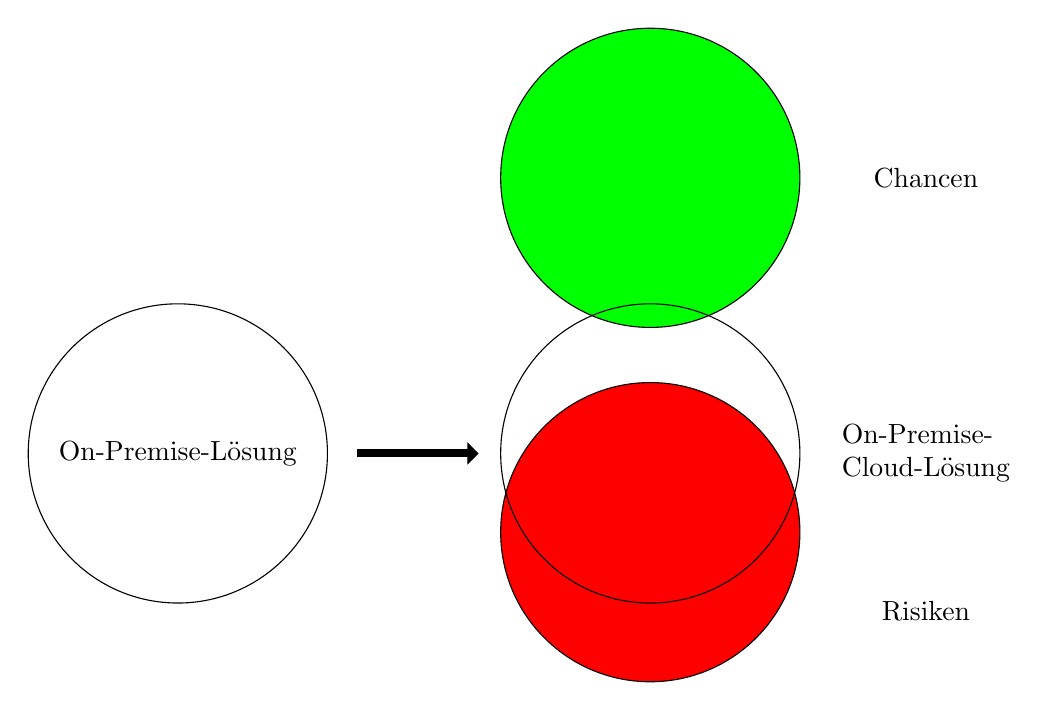
\begin{tikzpicture}
\newcommand{\rechts}{6}
\newcommand{\radius}{1.9cm}
\coordinate (centerTop) at (\rechts,3.5);
\coordinate (centerLinks) at (0,0);
\coordinate (centerRechts) at (\rechts,0);
\coordinate (centerBottom) at (\rechts,-1);

% Linker Kreis
\draw (centerLinks) circle (\radius) node [text=black] 
{On-Premise-Lösung};


% Oberer Kreis
\draw[fill=green] (centerTop) circle (\radius);
\node[align=left] at ($ (centerTop) + (3.5,0)$) {Chancen};

%Unterer Kreis mit Schrift
\draw[fill=red] (centerBottom) circle (\radius);
\node[align=left] at ($ (centerBottom) + (3.5,-1)$) {Risiken};


% Rechte Mitte
\draw (centerRechts) circle (\radius);
\node[align=left] at ($ (centerRechts) + (3.5,0)$) 
{\st{On-Premise-}\\Cloud-Lösung};

% Pfeil
\path[draw=black,solid,line width=1mm,fill=black,
preaction={-triangle 90,thin,draw,shorten >=-1mm}
] ($ (centerLinks) + (1.2 * \radius,0) $) -- ($ (centerRechts) + 
(-1.2 * \radius,0) $);

%\draw \secondcircle node [text=black,left] {On-Premise-Software};
%\draw \thirdcircle node [text=black,right] {$C$};
\end{tikzpicture}
\caption{Funktionsumfang vor und nach der Migration im Wasserfallmodell. 
Selbsterstellte Grafik.}
\label{fig:funktionsumfang_wasserfallmodell}
\end{center}
\end{figure}

In Abbildung~\ref{fig:funktionsumfang_wasserfallmodell} ist der Ansatz aus dem 
Fünf-Phasen-Modell dargestellt. Dabei wird die bestehende Anwendung in ihrem 
gesamten Umfang in die PaaS/SaaS-Cloud migriert und erst daran anschließend 
vermarktet. Dieser 1:1-Ansatz versteht -- zugespitzt formuliert -- unter einer 
Migration eine Umetikettierung des bestehenden Produktes.

Zumindest die Chance, eine agile Cloud-Lösung zu schaffen, die 
bereits früh einen Wert für den Kunden schafft und sich schnell an den 
Kundenwünschen orientiert weiterentwickelt, wird verschenkt. Der ISV 
läuft aber auch Gefahr weitere Vorteile nicht zu realisieren: Wenn er bei der 
Migration zunächst die Herstellung aller Funktionalitäten der Altsoftware in 
den Vordergrund stellt und dabei vernachlässigt, über Möglichkeiten 
nachzudenken, die Vorteile und Chancen der Cloud umzusetzen. Deshalb ist die 
Menge der Chancen nur zu einem geringen Teil in der Cloud-Lösung enthalten -- 
im Gegensatz zu den Risiken, die Teil der Cloud-Lösung werden, wenn man sich 
ihrer nicht bewusst ist und sie daher nicht vermeiden kann.

\usetikzlibrary{arrows}
\begin{figure}[h]
\begin{center}

\tikzset{
    %Define standard arrow tip
    >=stealth',
    %Define style for boxes
    punkt/.style={
           rectangle,
           %rounded corners,
           draw=black, very thick,
           text width=10em,
           minimum height=10em,
           text centered},
    % Define arrow style
    pil/.style={
           ->,
           very thick,
           shorten <=5pt,
           shorten >=5pt,},
    sepLine/.style={
	dashed,
	very thick
    }
}

\scalebox{1}{
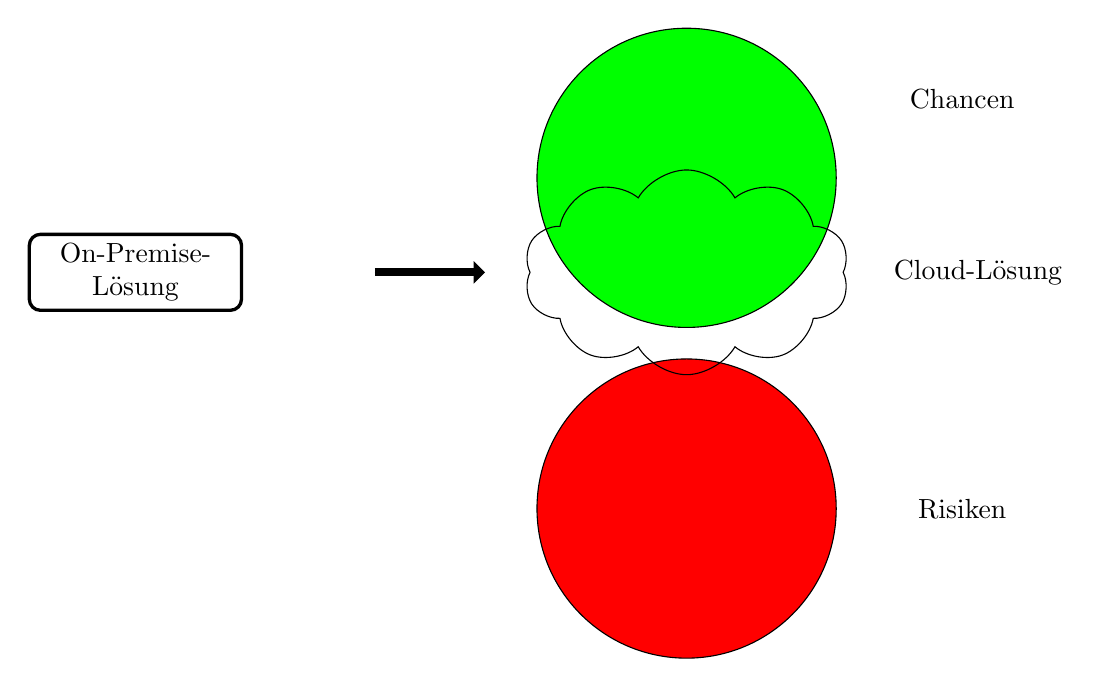
\begin{tikzpicture}
\newcommand{\rechts}{7}
\newcommand{\radius}{1.9cm}
\coordinate (centerTop) at (\rechts,1.2);
\coordinate (centerLinks) at (0,0);
\coordinate (centerRechts) at (\rechts,0);
\coordinate (centerBottom) at (\rechts,-3);

% Linker Kreis
%\draw (centerLinks) circle (1.5*\radius) node [text=black] 
%{On-Premise-Lösung};
\node[punkt] {On-Premise-Lösung} ; 

% Oberer Kreis
\draw[fill=green] (centerTop) circle (\radius);
\node[align=left] at ($ (centerTop) + (3.5,1)$) {Chancen};

%Unterer Kreis mit Schrift
\draw[fill=red] (centerBottom) circle (\radius);
\node[align=left] at ($ (centerBottom) + (3.5,0)$) {Risiken};


% Rechte Mitte
%\draw (centerRechts) circle (0.8*\radius);
\node[align=left] at ($ (centerRechts) + (3.7,0)$) {Cloud-Lösung};
\node [cloud, draw,cloud puffs=10,cloud puff arc=120, aspect=2, inner 
ysep=2em] (CLOUD) at (centerRechts) 
{};


% Pfeil
\path[draw=black,solid,line width=1mm,fill=black,
preaction={-triangle 90,thin,draw,shorten >=-1mm}
] ($ (centerLinks) + (1.6 * \radius,0) $) -- ($ (centerRechts) + 
(-1.4 * \radius,0) $);

%\draw \secondcircle node [text=black,left] {On-Premise-Software};
%\draw \thirdcircle node [text=black,right] {$C$};
\end{tikzpicture}
}
\caption{Funktionsumfang vor und nach der Migration nach dem in dieser Arbeit 
vorgestellten Vorgehensweise. 
Selbsterstellte Grafik.}
\label{fig:funktionsumfang_agil}
\end{center}
\end{figure}

Abbildung~\ref{fig:funktionsumfang_agil} zeigt die in dieser Arbeit 
vorgeschlagene Vorgehensweise. Hier ist die Cloud-Lösung in ihrem Umfang kleiner, 
als die bestehende On-Premise-Software, sodass sie gerade das 
enthält, was für die Vermarktung nötig ist. Die Beschränkung des Umfangs 
begünstigt eine schnelle Fertigstellung und Vermarktung. Fehlende Features 
werden agil nachentwickelt und in kurzen Abständen freigegeben. In der 
Cloud-Lösung werden von Anfang an Chancen maximiert und Risiken minimiert.

Im Ergebnis ist das hier vorgestellte Vorgehen weniger riskant, da nötige 
Investitionen geringer sind und Fehler wie Erfolge frühzeitig sichtbar werden. 
Darüber hinaus stehen in diesem Modell nicht die Kosteneinsparungen sondern strategische 
Ziele im Vordergrund. Da der zeitliche Horizont viel kleiner ist, kann 
die Wirtschaftlichkeitsprüfung weniger detailliert ausfallen. Es sollte 
lediglich geprüft geprüft werden, ob nötige Umsätze mit dem Funktionsumfang der 
Vision generiert werden können. 

Auf diesen letztgenannten Aspekt sollte ebenfalls die technische 
Machbarkeitsstudie abzielen: Kann auf der gewählten Cloud-Plattform ein vermarktbarer Teil des 
von der Produktvision vorgeschlagenen Leistungsumfangs implementiert werden? Dabei soll 
gerade nicht die gesamte Vision direkt umgesetzt werden. Sobald eine 
erste Version der Cloud-Lösung von Kunden genutzt wird, lässt sich erfragen 
oder ermitteln, wie die Entwicklung weitergehen soll; womöglich wird 
festgestellt, dass ein in der Vision vorgesehenes Feature gar keinen Anklang 
findet oder aber, dass die Vision in eine neue Richtung weiter gedacht werden 
muss.


\begin{comment}
\subsubsection{Technische Machbarkeit}


\subsubsection{Wirtschaftliche Machbarkeit}
"`In diesem Punkt unterscheidet sich Cloud-Computing von früheren Paradigmen
wie Outsourcing, welches nicht auf das Geschäftsmodell des Unternehmens wirken
will. Durch neue Anwendungsszenarien kann mit Cloud-Computing ein beachtlicher
Mehrwert geschaffen werden."' \pcite{}{154}{cloud_migration}

"`Alle Empfehlungen sollten mit einem Business Case hinterlegt werden, der
die Höhe der Kostenreduktion und die Verbesserung des Servicelevels zeigt."'
\pcite{}{158}{cloud_migration}
\end{comment}


\subsection{Phase III: Agiler, iterativer Entwicklungsprozess}
Die dritte Phase dieses Modells fasst die Phasen zwei bis fünf 
(Anforderungsanalyse und -Planung, Migration, Testen und Go-Live sowie 
Überwachung und Wartung) aus dem Fünf-Phasen-Modell zu einer Phase zusammen. In 
dieser Phase wird anstatt eines iterativen Wasserfallmodells ein agiles Modell verfolgt. Der Modellwechsel wird 
notwendig, weil sich in der Cloud die Art und Weise sowie der Rhythmus ändern, 
in der neue Versionen und Updates ausgeliefert werden. Bei konventioneller 
Software wurden Fehlerbehebungen häufig in Form kleiner Updates in festen 
Zyklen, beispielsweise halbjährlich ausgeliefert. Neue Funktionalitäten kamen 
hingegen in Form von neuen Softwareversionen (Upgrades) zum Kunden, für die 
erneut gezahlt werden musste. Im Cloud-Betrieb gibt es regelmäßig  nur eine 
Version der Software, in der nicht nur kontinuierlich Fehler behoben 
sondern auch neue Funktionen ergänzt werden, ohne, dass dies für die Nutzer mit 
Unterbrechungen verbunden wäre 
\pcite{}{}{changes_in_requirements_engineering,transitioning_to_saas}. Unter dieser Anforderung ist ein agiles Vorgehen im Sinne der Wettbewerbsfähigkeit 
besonders wichtig.

Der agile, iterative Entwicklungsprozess beginnt, wie in 
Abbildung~\ref{fig:vorgehensmodell} dargestellt, mit dem Requirements 
Engineering und der Produktvision als Input.

Das Requirements Engineering (Anforderungsmanagement) hat das Ziel 
Anforderungen eines Softwaresystems oder eines Features zu erheben, zu 
strukturieren, priorisieren und zu 
koordinieren. \pcite{}{}{changes_in_requirements_engineering} Auch die 
Identifizierung von Diskrepanzen zwischen Ergebnis und Ziel gehört dazu 
\pcite{}{}{requirements_engineering_process_for_saas_cloud_env}. Auch wenn sich 
an dieser Definition bei der Entwicklung in der Cloud nichts Grundsätzliches 
ändert, machen die Charakterisitika der Cloud doch ein Überdenken der Prozesse 
im Rahmen des Requirements Engineering notwendig 
\pcite{}{}{changes_in_requirements_engineering,transitioning_to_saas}.
Die Unterschiede zwischen Requirements Engineering bei On-Premise-Projekten im 
Vergleich zu SaaS-Projekten ist in Tabelle~\ref{tab:unterschiede_im_re} 
aufgeführt.
\begin{table}[ht!]
\centering
\begin{longtable}{|p{0.45\textwidth}|p{0.45\textwidth}|}
\hline
\textbf{On-Premise-Software} & \textbf{Software as a Service} \\
\hline %%%%%%%%%%%%%%%%%%%%%%%%%%%%%%%%%%%%%%%%%%%%%%%%%%%%%%%%%%%%%%%%%
Überschaubare Anzahl von Stakeholdern & Viele verschiedene Stakeholder \\
\hline
Keine oder geringe Einbeziehung des Kunden in die Entwicklung & Starke 
Einbeziehung des Kunden in die Entwicklung\\ \hline
Geschäftsbeziehung zum Kunden endet mit einmaliger Zahlung & langfristige 
Geschäftsbeziehung \\ \hline
Nutzungserfahrungen nur über spezielle Erhebungen & Direkte Rückmeldungen durch die Kunden, ggf.
motiviert durch die Hoffnung auf Fehlerbehebung oder neue Features \\ \hline
Regelmäßige, geplante Fehlerbehebung & Sofortige Fehlerbehebung \\ \hline
Keine neuen Features ohne Versionsupgrade & Andauernde Auslieferung neuer 
Features, ohne größere Verzögerung \\ \hline
Updates und Upgrades erfordern Downtime & Nahtloser Updateprozess ohne 
Unterbrechung \\ \hline
Upgrades haben größere Auswirkungen und machen Schulungen erforderlich & 
Kontinuierliche Auslieferung weniger disruptiv \\ \hline
Prognose und Test der Akzeptanz schwierig & Alternativen lassen sich an 
kleineren Nutzergruppen testen \\
\hline %%%%%%%%%%%%%%%%%%%%%%%%%%%%%%%%%%%%%%%%%%%%%%%%%%%%%%%%%%%%%%%%%
\end{longtable}
\caption{Unterschiede im Requirementsengineering. Entnommen aus 
\cite{changes_in_requirements_engineering}}
\label{tab:unterschiede_im_re}
\end{table}

Um auf die Änderungen im Requirements Engineering zu reagieren, sprechen 
\citeflow{changes_in_requirements_engineering} die folgenden Empfehlungen aus: Um auf sich schnell
ändernde Anforderungen reagieren zu können, sollte sich das Unternehmen intensiv mit aktuellen
Entwicklungen im Bereich agiler Methoden und der Anforderungsermittlung beschäftigen. Agile Methoden 
sind zwar keine besonderen Neuerungen der Cloud, sind aber aufgrund der vom Markt geforderten hohen Entwicklungsgeschwindigkeit geboten. Technisch kann die beschleunigte Entwicklung durch Mechanismen zur unterbrechungsfreien Auslieferung von Updates unterstützt werden. 
Bei der Anforderungsermittlung sollten Stakeholder mit systematischen Methoden identifiziert und priorisiert werden. Außerdem ist die Einbeziehung der Kunden mittels Feature Requests und Bug Reports essentiell um Vorteile aus der Cloud-Migration zu ziehen. Die Kunden sollen dabei das Gefühl bekommen, Einfluss auf die Entwicklung nehmen zu können. Dabei ebenfalls hilfreich ist Erhebung von Feedback. Dies kann entweder automatisch über gewonnene Nutzungsdaten geschehen, oder aber über Fragebögen. Ein Beispiel für das Potential der Cloud in diesem Bereich ist das Testen einer neuen Funktionalität an einer Testgruppe, die nichts von ihrer Teilnahme weiß. Anhand des Nutzungsverhaltens zeigt sich, ob die Neuerung intuitiv umgesetzt wurde. 


\begin{comment}
Aus \citepara{changes_in_requirements_engineering}
\begin{itemize}
	\item Bei einer Migration zu einem Service-Oriented-Architecture 
Modell, werden Teile aus einer Software geschnitten und über eine Schnittstelle 
als Dienstleistung angeboten. Daher wird in der Regel versucht, die meisten 
Funktionalitäten zu übernehmen. Für mehr Informationen: 
\pcite{}{}{service-oriented_migration}
	\item Es gibt drei Nicht-Funktionale Anforderungen die aus SaaS 
entstehen: 
\begin{enumerate}
	\item Software muss in einer Cloud-Umgebung gehostet werden. Dies 
hat Einfluss auf die Themen Sicherheit, Vertraulichkeit, Verschwiegenheit, 
Compliance.
	\item In der Regel eine webbasierte Anwendung, d.h. es werden übliche 
Internetprotokolle verwendet. Dies hat Einfluss auf die Themen: Multi-Tenancy, 
User Concurrency, Konfigurierbarkeit, Skalierbarkeit, Verlässlichkeit, 
Leistungsfähigkeit, Verfügbarkeit, Kompatibilität, Interoperabilität, 
Portabilität, Effizienz, Direktheit
	\item In der Regel ist eine Bedienung über den Browser möglich, die 
Installation einer zusätzlichen Anwendung nicht erforderlich
\end{enumerate}
	\item \pcite{}{}{requirements_engineering_process_for_saas_cloud_env} 
Neuer Stakeholder: Cloud Service Provider. Schlagen Checkliste für neue 
Stakeholder vor.
	\item Noch mehr Stakeholder Analysten, Grafik Designer, Kunden, 
Marketing, Sicherheitsexperten 
\pcite{}{}{adapting_the_software_engineering_process}
\end{itemize}


\subsubsection{Kategorien und Anforderungen}
Aus \citeflow{requirements_engineering_process_for_saas_cloud_env}:
\begin{description}
	\item[Anforderungen an die Architektur] Passendes Auslieferungsmodell, 
Sicherheit, Privatsspähre, Hohe Verfügbarkeit und Anpassbarkeit. Verschiedene 
Levels von Service Level Agreements (SLA). Sollte zustandslos (niedrige Kosten, 
hohe Zuverlässigkeit und Performanz) sein. Fehlertolerant, umfassende 
Redundanz und Uptime, Strategien für den Fehlerfall. Wiederbenutzbare 
Komponenten. Integration mit Altsystemen, API Anforderungen. 
	\item[Anforderungen aus dem Operativen/an das Verhalten] Leichte 
Anpassbarkeit und Erweiterbarkeit der Interfaces, Daten- und Businessprozesse, 
User Experience, Designanforderungen, Sicherheit und Privatsspähre, 
Verfügabarkeit, Performanz, Interoperabilität, häufige und nicht unterbrechende 
Upgrades. Kapazitätsplanung, Datenmigration, 
	\item[Anforderungen des Managements] Zentralisierte Berichte, 
Monitoring über Einhaltung der SLAs, Rechnungen, Hosting, User Management, 
Kapazitätsplanung und Zuteilung, Datenmanagement, Speicherung, Verarbeitung
	\item[Anforderungen aus Technik/Implementierung] Recruitment, 
Rollenwechsel, 
\end{description}

Schritte, die laut 
\citeflow{requirements_engineering_process_for_saas_cloud_env} im klassischen 
Requirements Engineering ergänzt werden sollten:
\begin{description}
	\item[Testen der Eignung der Cloud-Architektur mit initialen 
Anforderungen]
	\item[Public oder Private Cloud?]
	\item[Passende Cloud Service Provider identifizieren]
	\item[Kosten der Cloud-Lösung abschätzen] Cloudonomics
	\item[Anforderungen dokumentieren] Wekcge Art von physischer und 
persönlicher Sicherheit bietet die CLoud? Wie würden Anwendungen überwacht, die 
in einer Public Cloud? Wie skalierbar wäre die Cloud?
\end{description}

\begin{comment}
\subsubsection{Anforderungsermittlung}
\subsubsection{Return on Investment (ROI)}
\subsubsection{Total Cost of Ownership (TCO)}



\begin{comment}
\label{cha:entwicklung}
Dieses Kapitel dient der Entwicklung eines konzeptuellen Rahmens auf Basis theoretischer Grundlagen, vorausgesetzt sie verfolgen einen positivistischen Ansatz. Hierfür leiten Sie Hypothesen aus verschiedenen sinnvoll kombinierten Quellen her. Hierdurch generieren Sie aus bestehendem Wissen neues Wissen, was eine Eigenleistung und somit ein wichtiger Bestandteil Ihrer Arbeit darstellt.

Sollte Ihre Arbeit nicht positivistisch ausgelegt sein, stellt dieser Abschnitt kein Pflichtkapitel der Arbeit dar. Alternativ beschreiben Sie Anforderungen für ein mögliches Konzept oder verzichten vollständig auf dieses Kapitel.

\textbf{Setzen Sie sich frühzeitig mit Ihrem Betreuer in Verbindung, um Ihre Gliederung abzustimmen und mögliche Missverständnisse zu beseitigen.}

Im Folgenden werden einige allgemeine Hinweise zu den Themen richtiges Zitieren und Literaturrecherche gegeben.


\subsection{Quellen und richtiges Zitieren}
Quellen können in Fußnote oder direkt im Text platziert werden. Alles was nicht Ihr eigenes Gedankengut darstellt, muss mit einer entsprechenden Quelle belegt werden. Hierbei können wörtliche und indirekte Zitate verwendet werden. Wörtliche Zitate sind immer mit der Seitennummer der Quelle anzugeben.

Beispiel für ein direktes Zitat:

%\textit{\glqq The case study is a research strategy which focuses in understanding the dynamics present within single settings\grqq} \pcite{}{543}{eisenhardt1989}.

Beispiel für ein indirektes Zitat:

%Eine explorative Fallstudie dient der Gewinnung von neuen Erkenntnissen und der Bildung von neuen Hypothesen über bestimmte Sachverhalte. Durch den Beitrag zum Theorieaufbau ist der Erkenntnisgewinn höher als bei einer reinen deskriptiven Fallstudie. In explorativen Fallstudien werden Phänomene in noch wenig erforschten Gebieten identifiziert und aus erkannten Zusammenhängen neue Hypothesen gebildet \citepara{eisenhardt1989}.

Alternativ kann die Quelle auch im  laufenden Text angegeben werden:

%Nach \citeflow{eisenhardt1989} wird die Wichtigkeit der Fallauswahl oft unterschätzt. Die Fälle können zwar zufällig ausgewählt werden, dies ist aber weder notwendig noch wünschenswert.

Quellenangaben bestehen aus Autor, Jahr und ggf. Seitenangabe. Bei zwei Autoren sind beide Autoren zu nennen, bei mehreren Autoren nur der erste Autor mit dem Zusatz „et al.“.\newpage


\subsection{Zitieren mit Endnoten}
Im Rahmen der Erstellung von Arbeiten am Fachgebiet ISE ist das Literaturverwaltungsprogramm EndNote zu verwenden. Dieses steht auf der \href{http://www.ulb.tu-darmstadt.de/service/literaturverwaltung_start/endnote_ulb/endnote.de.jsp
}{ULB-Seite} zum Download verfügbar.


\subsubsection{Lateinischer Text mit Zitaten für Erstellung des Literaturverzeichnisses}
\label{cha:source:latintext}
%Lorem ipsum dolor sit amet, consectetur adipiscing elit. Sed vitae lacus eu
%augue semper lobortis vitae aliquet leo. Fusce eleifend sodales commodo
%\citepara{eisenhardt1989}. Mauris arcu metus, bibendum sagittis condimentum
%eget, placerat a enim \citepara{baechle2010}. Quisque sit amet sagittis lectus.
%Curabitur sit amet libero eu felis elementum mollis. Nullam odio diam, mollis
%vitae viverra ut, laoreet ut odio. Praesent facilisis suscipit consequat. Morbi
%feugiat rutrum erat, eu sagittis nibh rhoncus nec \citepara{melao2000}.

%In euismod, arcu ut semper adipiscing, nibh odio ullamcorper arcu, ut scelerisque massa magna nec quam \citepara{benlian2013}. Curabitur bibendum nibh eget augue pellentesque iaculis \citepara{sheffi2005}. Praesent iaculis auctor gravida. Quisque congue, magna ut bibendum semper, enim tortor ultrices lorem, ac feugiat tortor lectus nec nunc \citepara{carnap1974}. Pellentesque habitant morbi tristique senectus et netus et malesuada fames ac turpis egestas. Lorem ipsum dolor sit amet, consectetur adipiscing elit. Fusce dignissim, augue a sodales tristique, neque dui mollis arcu, id interdum augue justo sed lacus \citepara{welchering2013}. Vestibulum ante ipsum primis in faucibus orci luctus et ultrices posuere cubilia Curae; Mauris euismod bibendum nulla, sed accumsan urna tempor sed. Etiam eget diam eros, sed aliquet dolor \citepara{broadbent1996}. Phasellus vitae quam in orci convallis pharetra. Donec sit amet imperdiet nisi \citepara{kayser2013}. Sed vel interdum orci. Praesent vulputate, dolor id varius egestas, enim libero cursus neque, a cursus sapien nulla ut augue. Nullam vitae tortor nisl, vitae cursus enim. Suspendisse eget metus ipsum, sit amet varius sem \citepara{shazly2013}.

\subsection{Literaturrecherche}
Anbei eine kurze Auflistung von möglichen Kanälen zur Literaturrecherche.

\textbf{Zu Verwaltung Ihrer Literatur benutzen Sie bitte das Programm EndNote, dieses wird kostenfrei von der TU zu Verfügung gestellt.}

\url{http://www.ulb.tu-darmstadt.de/angebot/service/literaturverwaltung/endnote.de.jsp}

\subsubsection{Angebot der ULB}
\begin{itemize}
\item Universitätsbibliotheken (\url{http://www.ulb.tu-darmstadt.de/})
\item Rechercheangebot der ULB (\url{http://www.ulb.tu-darmstadt.de/recherche/})
\end{itemize}

\subsubsection{Online-Datenbanken und -Bibliotheken}
\begin{itemize}
\item Elektronische Zeitschriftenbibliothek (EZB) \\
(\url{http://rzblx1.uni-regensburg.de/ezeit/fl.phtml?bibid=TUDA})
\item AIS Electronic Library (AISeL)\\
(\url{http://aisel.aisnet.org/})
\item Zeitschriftendatenbank (ZDB)\\
(\url{http://dispatch.opac.ddb.de/DB=1.1/srt=YOP/})
\item Datenbank-Infosystem (DBIS): Literatur- und Fakten-Datenbank\\
(\url{http://rzblx10.uni-regensburg.de/dbinfo/fachliste.php?bib_id=tud})
\item IEEE Xplore \\
(\url{http://ieeexplore.ieee.org/Xplore/dynhome.jsp?tag=1})
\item EBSCO: internationale wirtschafts-wiss. Zeitschriften\\ (\url{http://search.ebscohost.com})
\item Springer-Online: Bücher/Beiträge des Springer Verlags\\
(\url{http://www.springerlink.com})
\item WiSo Net: deutschsprachige Literatur zu Wirtschafts- und Sozialwissenschaften\\
(\url{www.wiso-net.de})

\end{itemize}

\subsubsection{Sonstiges}
\begin{itemize}
\item \textbf{Google Scholar:} Suchdienst für wissenschaftliche Recherchen (http://scholar.google.de)
\item \textbf{Verlagswebseiten} Recherche und den Zugriff auf Zeitschriften- und Zeitungsartikel und E-Books
\item \textbf{Webseiten von Unternehmen} für die Recherche von Unternehmensdaten und-statistiken sowie Unternehmensdatenbanken
\item \textbf{Webseiten von Bundes- und Landesbehörden sowie der EU}
 Statistisches Bundesamt (http://www.destatis.de)
\\Presse- und Informationsamt der Bundesregierung (http://www.bundesregierung.de)
\item \textbf{Webseiten von Marktforschungsinstituten}
(für Marktanteile und Verbraucheranalysen)
\item \textbf{Webseiten von Verbänden und Kammern}
Institut der deutschen Wirtschaft (http://www.deutsche-wirtschaft.de)
\end{itemize}
\end{comment}
